\section{eo\-String$<$ fitness\-T $>$ Class Template Reference}
\label{classeo_string}\index{eoString@{eoString}}
Adaptor that turns an STL std::string into an {\bf EO}{\rm (p.\,\pageref{class_e_o})}.  


{\tt \#include $<$eo\-String.h$>$}

Inheritance diagram for eo\-String$<$ fitness\-T $>$::\begin{figure}[H]
\begin{center}
\leavevmode
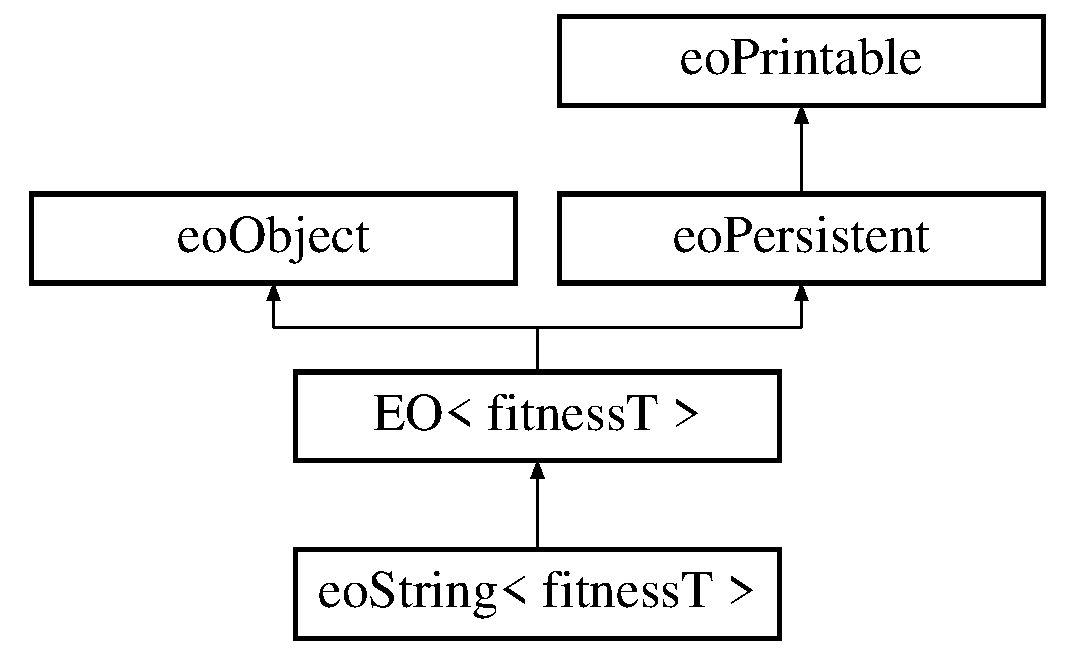
\includegraphics[height=4cm]{classeo_string}
\end{center}
\end{figure}
\subsection*{Public Types}
\begin{CompactItemize}
\item 
typedef char {\bf Type}\label{classeo_string_w0}

\item 
typedef char {\bf Atom\-Type}\label{classeo_string_w1}

\item 
typedef std::string {\bf Container\-Type}\label{classeo_string_w2}

\end{CompactItemize}
\subsection*{Public Member Functions}
{\bf }\par
\begin{CompactItemize}
\item 
{\bf eo\-String} (const std::string \&\_\-str=\char`\"{}\char`\"{})\label{classeo_string_z24_0}

\begin{CompactList}\small\item\em ctor \item\end{CompactList}\item 
virtual void {\bf print\-On} (std::ostream \&os) const \label{classeo_string_z24_1}

\begin{CompactList}\small\item\em printing... \item\end{CompactList}\end{CompactItemize}

\begin{Indent}{\bf Methods from eo\-Object}\par
{\em read\-From and print\-On are directly inherited from eo1d }\begin{CompactItemize}
\item 
virtual std::string {\bf class\-Name} () const 
\begin{CompactList}\small\item\em Inherited from {\bf eo\-Object}{\rm (p.\,\pageref{classeo_object})}. \item\end{CompactList}\end{CompactItemize}
\end{Indent}


\subsection{Detailed Description}
\subsubsection*{template$<$class fitness\-T$>$ class eo\-String$<$ fitness\-T $>$}

Adaptor that turns an STL std::string into an {\bf EO}{\rm (p.\,\pageref{class_e_o})}. 



Definition at line 42 of file eo\-String.h.

\subsection{Member Function Documentation}
\index{eoString@{eo\-String}!className@{className}}
\index{className@{className}!eoString@{eo\-String}}
\subsubsection{\setlength{\rightskip}{0pt plus 5cm}template$<$class fitness\-T$>$ virtual std::string {\bf eo\-String}$<$ fitness\-T $>$::class\-Name (void) const\hspace{0.3cm}{\tt  [inline, virtual]}}\label{classeo_string_z26_0}


Inherited from {\bf eo\-Object}{\rm (p.\,\pageref{classeo_object})}. 

\begin{Desc}
\item[See also:]{\bf eo\-Object}{\rm (p.\,\pageref{classeo_object})} \end{Desc}


Reimplemented from {\bf EO$<$ fitness\-T $>$} {\rm (p.\,\pageref{class_e_o_z10_0})}.

Definition at line 74 of file eo\-String.h.

The documentation for this class was generated from the following file:\begin{CompactItemize}
\item 
eo\-String.h\end{CompactItemize}
